\documentclass{ximera}

\begin{document}
	\author{Stitz-Zeager}
	\xmtitle{Vectors}{}

\mfpicnumber{1}

\opengraphsfile{Vectors}

\setcounter{footnote}{0}

\label{Vectors}

As we have seen numerous times in this book, Mathematics can be used to model and solve real-world problems.  For many applications, real numbers suffice; that is, real numbers with the appropriate units attached can be used to answer questions like ``How close is the nearest Sasquatch nest?''   

 

There are other times though, when these kinds of quantities do not suffice.  Perhaps it is important to know, for instance, how close the nearest Sasquatch nest is as well as the direction in which it lies.  To answer questions like these which involve both a quantitative answer, or \textit{magnitude}, along with a \textit{direction}, we use the mathematical objects called \index{vector ! definition of}\textbf{vectors}.\footnote{The word `vector' comes from the Latin \textit{vehere} meaning `to convey' or `to carry.'}    

 

A vector is represented geometrically as a directed line segment where the magnitude of the vector is taken to be the length of the line segment and the direction is made clear with the use of an arrow at one endpoint of the segment.   When referring to vectors in this text, we shall adopt\footnote{Other textbook authors use bold vectors such as $\textbf{v}$.  We find that writing in bold font on the chalkboard is inconvenient at best, so we have chosen the `arrow' notation.} the `arrow' notation, so the symbol  $\overrightarrow{v}$ is read as `the vector $v$'. Below in blue is a typical vector $\overrightarrow{v}$ with endpoints $P\left(1, 2\right)$ and $Q\left(4, 6\right)$. 

 

The point $P$  is called the \index{vector ! initial point}\textit{initial point} or \index{vector ! tail}\textit{tail} of  $\overrightarrow{v}$ and the point $Q$ is called the \index{vector ! terminal point}\textit{terminal point} or \index{vector ! head}\textit{head} of  $\overrightarrow{v}$.   Since we can reconstruct $\overrightarrow{v}$ completely from $P$ and $Q$, we write $\overrightarrow{v} = \overrightarrow{PQ}$, where the order of points $P$ (initial point) and $Q$ (terminal point) is important. (Think about this before moving on.)

\begin{center} 
\geogebra{gnqhdrwr}{800}{600} 
\end{center}

While it is true that $P$ and $Q$ completely determine $\overrightarrow{v}$, it is important to note that since vectors are defined in terms of their two characteristics,  magnitude and direction, any directed line segment with the same length and direction as $\overrightarrow{v}$ is considered to be the same vector as $\overrightarrow{v}$, regardless of its initial point.

 In the case of our vector $\overrightarrow{v}$ above, any vector which moves three units to the right and four up\footnote{If this idea of `over' and `up' seems familiar, it should.  The slope of the line segment containing $\overrightarrow{v}$ is  $\frac{4}{3}$.} from its initial point to arrive at its terminal point is considered the same vector as $\overrightarrow{v}$.  The notation we use to capture this idea is the \index{vector ! component form} \textit{component form} of the vector, $\overrightarrow{v} = \left<3,4\right>$, where the first number, $3$, is called the $x$-\textit{component} \index{vector ! $x$-component} of $\overrightarrow{v}$ and the second number, $4$, is called the $y$-\textit{component} \index{vector ! $y$-component} of $\overrightarrow{v}$\footnote{Note that there are a number of other notations for vectors.  In fact, the Geogebra code to draw this vector uses the form 
$\overrightarrow{v} = \left(\begin{array}{cc}
3 \\ 4 \end{array}\right).$}.  
 
 For example, if we wanted to reconstruct $\overrightarrow{v} = \left<3,4\right>$ with initial point $P'(-2,3)$, then we would find the terminal point of $\overrightarrow{v}$ by adding $3$ to the $x$-coordinate and adding $4$ to the $y$-coordinate to obtain the terminal point $Q'(1,7)$, as seen below if we set $a=-2$ and $b=3$.

\begin{center} 
\geogebra{zp9vptmw}{800}{600} 
\end{center}

The component form of a vector is what ties these very geometric objects back to Algebra and ultimately Trigonometry.  We generalize our example in our definition below.

%% \colorbox{ResultColor}{\bbm
\begin{definition} \label{componentformvector}  Suppose $\overrightarrow{v}$ is represented by a directed line segment with initial point $P\left(x_0, y_0\right)$ and terminal point $Q\left(x_1, y_1\right)$.  The \textbf{component form} of $\overrightarrow{v}$ is given by \index{component form of a vector}

\[ \overrightarrow{v} = \overrightarrow{PQ} = \left< x_1 - x_0, y_1 - y_0 \right> \]


\end{definition}
%% \ebm}

 

Using the language of components, we have that two vectors are equal if and only if their corresponding components are equal.  That is, $\left<v_1, v_2\right> = \left<v_1', v_2'\right>$ if and only if $v_1 = v_1'$ and $v_2 = v_2'$. (Again, think about this before reading on.)  

 

We now set about defining operations on vectors.  Suppose we are given two vectors $\overrightarrow{v}$ and $\overrightarrow{w}$.  The sum, or \index{vector ! resultant} \textit{resultant} vector $\overrightarrow{v} + \overrightarrow{w}$ is obtained as follows.  First, plot $\overrightarrow{v}$.  Next, plot $\overrightarrow{w}$ so that its initial point is the terminal point of $\overrightarrow{v}$.  To plot the vector $\overrightarrow{v} + \overrightarrow{w}$ we begin at the initial point of $\overrightarrow{v}$ and end at the terminal point of $\overrightarrow{w}$.  It is helpful to think of the vector $\overrightarrow{v} + \overrightarrow{w}$ as the `net result' of moving along $\overrightarrow{v}$ then moving along $\overrightarrow{w}$.

\begin{center} 
\geogebra{wevqxuzp}{800}{600} 
\end{center}

Our next example makes good use of resultant vectors and reviews bearings and the Law of Cosines.\footnote{If necessary, review Sections \ref{bearings} and \ref{TheLawofCosines}.}  


\begin{example} \label{vectorbearingex}  A plane leaves an airport with an airspeed\footnote{That is, the speed of the plane relative to the air around it. If there were no wind, plane's airspeed would be the same as its speed as observed from the ground.  How does wind affect this?  Keep reading!}  of 175 miles per hour at a  bearing of  N$40^{\circ}$E.  A 35 mile per hour wind is blowing at a bearing of S$60^{\circ}$E.  Find the true speed of the plane, rounded to the nearest mile per hour,  and the true bearing of the plane, rounded to the nearest degree.

{\bf Solution:} For both the plane and the wind, we are given their speeds and their directions.  Coupling speed (as a magnitude) with direction is the concept of \textit{velocity} which we've seen a few times before.\footnote{See Section \ref{circularmotion}, for instance.} 

 

We let $\overrightarrow{v}$ denote the plane's velocity and $\overrightarrow{w}$ denote the wind's velocity in the diagram below.   The `true' speed and bearing is found by analyzing the resultant vector, $\overrightarrow{v} + \overrightarrow{w}$.  

 

From the vector diagram, we get a triangle, the lengths of whose sides are the magnitude of $\overrightarrow{v}$, which is 175, the magnitude of $\overrightarrow{w}$, which is 35, and the magnitude of $\overrightarrow{v} + \overrightarrow{w}$, which we'll call $c$. 

 

From the given bearing information, we go through the usual geometry to determine that the angle between the sides of length 35 and 175 measures $100^{\circ}$. 


\begin{center}
\begin{tabular}{cc}

%================ LEFT FIGURE =====================
\begin{tikzpicture}[scale=0.75,font=\large,
    >=Latex,
    line cap=round,
    line join=round]

% Axes
\draw[->,line width=1.2pt] (-0.5,0)--(8.5,0) node[right] {\scriptsize E};
\draw[->,line width=1.2pt] (0,-1.5)--(0,9) node[above] {\scriptsize N};

% Vectors
\draw[->,line width=1.5pt] (0,0)--(6.43,7.66)
    node[pos=1.05,left] {\scriptsize $\overrightarrow{v}$};

\draw[->,line width=1.5pt] (0,0)--(1.73,-1)
    node[pos=.99,below] {\scriptsize $\overrightarrow{w}$};

% Construction lines
\draw[dashed,->] (0,0)--(8.16,6.66);
\draw[dotted] (1.73,-1)--(8.16,6.66);
\draw[dotted] (6.43,7.66)--(8.16,6.66);

\node[right] at (8.16,6.66)
    {\scriptsize $\overrightarrow{v}+\overrightarrow{w}$};

% Angle arcs
\draw[->] (85:5) arc (85:55:5);
\node at (1.88,5.17) {\scriptsize $40^\circ$};

\draw[->] (275:1.5) arc (275:325:1.5);
\node at (1,-1.73) {\scriptsize $60^\circ$};

\end{tikzpicture}

&
\hspace{0.75in}

%================ RIGHT FIGURE =====================
\begin{tikzpicture}[scale=0.75,font=\large,
    >=Latex,
    line cap=round,
    line join=round]

% Axes
\draw[->,line width=1.2pt] (-0.5,0)--(8.5,0) node[right] {\scriptsize E};
\draw[->,line width=1.2pt] (0,-1.5)--(0,9) node[above] {\scriptsize N};

% Triangle
\draw[line width=1.5pt]
    (0,0)--(6.43,7.66)--(8.16,6.66)--cycle;

% Dotted reference lines
\draw[dotted] (0,0)--(1.73,-1);
\draw[dotted] (5.93,7.66)--(6.93,7.66);
\draw[dotted] (6.43,7.15)--(6.43,8.17);

% Side labels
\node at (3,4.5) {\scriptsize 175};
\node at (5,3.5) {\scriptsize $c$};
\node at (7.5,7.5) {\scriptsize 35};

% Angle arcs
\draw[->] (85:3) arc (85:55:3);
\node at (1.2,3.3) {\scriptsize $40^\circ$};

\draw[->] (275:1.5) arc (275:325:1.5);
\node at (1,-1.73) {\scriptsize $60^\circ$};

\draw[<->] ($(6.43,7.66)+({cos(235)},{sin(235)})$)
    arc (235:325:1);
\node at (6.5,6.25) {\scriptsize $100^\circ$};

\draw[<->] (41:5) arc (41:49:5);
\node at (3.9,3.9) {\scriptsize $\alpha$};

\end{tikzpicture}

\end{tabular}
\end{center}

From the Law of Cosines, we determine $c = \sqrt{31850 - 12250\cos(100^{\circ})} \approx 184$, which means the true speed of the plane is (approximately) $184$ miles per hour. 

 

 To determine the true bearing of the plane, we need to determine the angle $\alpha$.  Using the Law of Cosines once more,\footnote{Or, since our given angle, $100^{\circ}$, is obtuse, we could use the Law of Sines without any ambiguity here.} we find $\cos(\alpha) = \frac{c^2+29400}{350c}$ so that $\alpha \approx 11^{\circ}$.  
 
  
 
 Given the geometry of the situation, we add $\alpha$ to the given $40^{\circ}$ and find the true bearing of the plane to be (approximately) N$51^{\circ}$E. \qed

\end{example}

Our next step is to define addition of vectors component-wise to match the geometric action.\footnote{Adding vectors `component-wise' should seem hauntingly familiar.  Compare this with how matrix addition was defined in section \ref{MatArithmetic}. In more advanced courses. chief among them Linear Algebra, vectors are actaually \textit{defined} as $1\times n$ or $n \times 1$ matrices, depending on the situation.}

 

%% \colorbox{ResultColor}{\bbm
\begin{definition} \label{vectoradd}  Suppose $\overrightarrow{v} = \left<v_1,v_2\right>$ and $\overrightarrow{w} = \left<w_1,w_2\right>$.  The vector $\overrightarrow{v} + \overrightarrow{w}$ is defined by \index{vector ! addition ! definition of}

\[ \overrightarrow{v} + \overrightarrow{w}  = \left< v_1 + w_1, v_2 + w_2 \right> \]


\end{definition}
%% \ebm}

\begin{example}  \label{vectoraddex}  Let  $\overrightarrow{v} = \left<3,4\right>$ and suppose  $\overrightarrow{w} = \overrightarrow{PQ}$ where $P(-3,7)$ and $Q(-2,5)$.  Find $\overrightarrow{v} + \overrightarrow{w}$ and interpret this sum geometrically.

\medskip

{\bf Solution.}  Before can add the vectors using Definition \ref{vectoradd}, we need to write  $\overrightarrow{w}$ in component form. Using Definition \ref{componentformvector}, we get $\overrightarrow{w} = \left<-2-(-3),5-7\right> = \left<1,-2\right>$.  Thus,

  \[\overrightarrow{v} + \overrightarrow{w} =  \left<3,4\right> + \left<1,-2\right> =  \left< 3 + 1, 4 + (-2) \right> =  \left<4, 2\right>. \]
                                        
To visualize this sum, we draw $\overrightarrow{v}$ with its initial point at $(0,0)$ (for convenience) so that its terminal point is $(3,4)$.  Next, we graph $\overrightarrow{w}$ with its initial point at $(3,4)$.  Moving one to the right and two down, we find the terminal point of $\overrightarrow{w}$ to be $(4,2)$.  

\begin{center} 
\geogebra{rqhjc7ev}{800}{600} 
\end{center}

We see the vector $\overrightarrow{v} + \overrightarrow{w}$ has initial point $(0,0)$ and terminal point $(4,2)$ so its component form  is $\left<4,2\right>$. \qed

\end{example}

In order for vector addition to enjoy the same kinds of properties as real number addition, it is necessary to extend our definition of vectors to include a `zero vector', $\overrightarrow{0} = \left<0, 0\right>$.  

Geometrically,  $\overrightarrow{0}$ represents a point, which we can (very broadly) think of as a directed line segment with the same initial and terminal points.  The reader may well object to the inclusion of $\overrightarrow{0}$, since after all, vectors are supposed to have both a magnitude (length) and a direction.

While it seems clear that the magnitude of $\overrightarrow{0}$ should be $0$, it is not clear what its direction is.  As we shall see, the direction of $\overrightarrow{0}$ is in fact undefined, but this minor hiccup in the natural flow of things is worth the benefits we reap by including $\overrightarrow{0}$ in our discussions.  We have the following theorem.

%% \colorbox{ResultColor}{\bbm
\begin{theorem} \label{vectoradditionprops}  \textbf{Properties of Vector Addition} \index{vector ! addition ! properties of}
\begin{itemize}

\item  \textbf{Commutative Property:}  For all vectors $\overrightarrow{v} \text{ and } \overrightarrow{w}$, $\overrightarrow{v} + \overrightarrow{w} = \overrightarrow{w} + \overrightarrow{v}$. \index{vector ! addition ! commutative property}\index{commutative property ! vector ! addition}

\item  \textbf{Associative Property:}  For all vectors $\overrightarrow{u}, \overrightarrow{v} \text{ and } \overrightarrow{w}$, $\left(\overrightarrow{u} + \overrightarrow{v}\right) + \overrightarrow{w} = \overrightarrow{u} + \left(\overrightarrow{v} + \overrightarrow{w}\right)$. \index{vector ! addition ! associative property}\index{associative property ! vector ! addition}

\item  \textbf{Identity Property:} \index{vector ! additive identity}  For all vectors $\overrightarrow{v}$,  \[\overrightarrow{v} + \overrightarrow{0} = \overrightarrow{0} + \overrightarrow{v} = \overrightarrow{v}.\] 

The vector $\overrightarrow{0}$ acts as the additive identity for vector addition. 

\item  \textbf{Inverse Property:} \index{vector ! additive inverse}  For every vector  $\overrightarrow{v} = \left< v_1, v_2 \right>$, the vector $\overrightarrow{w} = \left< - v_1, -v_2 \right>$ satisfies  \[\overrightarrow{v} + \overrightarrow{w} = \overrightarrow{w} + \overrightarrow{v} = \overrightarrow{0}.\] 

That is, the additive inverse of a vector is the vector of the additive inverses of its components.

\end{itemize}
\end{theorem}
%% \ebm}


The properties in Theorem \ref{vectoradditionprops} are easily verified using the definition of vector addition,\footnote{The interested reader is encouraged to compare Theorem \ref{vectoradditionprops} and the ensuing discussion with Theorem \ref{matrixadditionprops} in Section \ref{MatArithmetic}.}  and are a direct consequence of the definition of vector addition along with properties inherited from real number arithmetic.

For the commutative property, we note that if $\overrightarrow{v} = \left<v_1,v_2\right>$ and $\overrightarrow{w} = \left<w_1,w_2\right>$ then

\[ \begin{array}{rcl} \overrightarrow{v} + \overrightarrow{w}  & = &  \left< v_1, v_2 \right> +  \left<  w_1, w_2 \right> \\
& = & \left< v_1 + w_1, v_2 + w_2 \right> \\
& = &  \left< w_1 + v_1, w_2 + v_2 \right> \\
& = & \overrightarrow{w} + \overrightarrow{v} \end{array} \]

Geometrically, we can `see' the commutative property by realizing that the sums $\overrightarrow{v}+\overrightarrow{w}$ and $\overrightarrow{w} + \overrightarrow{v}$ are the same directed diagonal determined by the parallelogram below.

\begin{center} 
\geogebra{dnfpqykt}{800}{600} 
\end{center}

The proofs of the associative and identity properties proceed similarly, and the reader is encouraged to verify them and provide accompanying diagrams.  

The additive identity property is likewise verified algebraically using a calculation.  If $\overrightarrow{v} = \left<v_1,v_2\right>$ , then

 \[ \overrightarrow{v} + \overrightarrow{0} = \left<v_1,v_2\right> + \left<0, 0\right> = \left< v_1 + 0, v_2 + 0 \right> =  \left<v_1,v_2\right>  = \overrightarrow{v}.\]
 
 From the commutative property of vector addition, we get that $\overrightarrow{0} + \overrightarrow{v} = \overrightarrow{v}$ as well.  Again, the reader is encouraged to visualize what this means geometrically.\footnote{Recall, $\overrightarrow{0}$ is represented geometrically as a point \ldots}

Regarding additive inverses, we can verify by direct computation that if $\overrightarrow{v} = \left< v_1, v_2 \right>$ and  $\overrightarrow{w} = \left< - v_1, -v_2 \right>$, 

\[ \overrightarrow{v} + \overrightarrow{w} = \left< v_1, v_2 \right> + \left< - v_1, -v_2 \right> = \left<  v_1 + ( - v_1), v_2 + ( - v_2) \right> = <0,0> = \overrightarrow{0}.\]

Once again, the commutative property of vector addition assures us  that, likewise, $\overrightarrow{w} + \overrightarrow{v} = \overrightarrow{0}$.

Moreover, additive inverses of vectors are \textit{unique}.    That is, given a vector $\overrightarrow{v} = \left<v_1, v_2\right>$, there is precisely only \textit{one} vector $\overrightarrow{w}$ so that $\overrightarrow{v} + \overrightarrow{w} = \overrightarrow{0}$.

To see this, suppose a vector $\overrightarrow{w} = \left<w_1,w_2\right>$ satisfies  $\overrightarrow{v} + \overrightarrow{w} = \overrightarrow{0}$.  By the definition of vector addition, we have $\left<v_1 + w_1, v_2 + w_2\right> = \left<0,0\right>$.  Hence, $v_1 + w_1 = 0$ and $v_2 + w_2 = 0$.  We get $w_1 = -v_1$ and $w_2  = -v_2 $ so that $\overrightarrow{w} = \left<-v_1 , -v_2 \right>$ as prescribed in Theorem \ref{vectoradditionprops}.  

Hence, every vector $\overrightarrow{v}$ has one, and only one, additive inverse.  In general, we denote the additive inverse of a vector $\overrightarrow{v}$ with the (highly suggestive) notation $- \overrightarrow{v}$.

 Geometrically, the vectors $\overrightarrow{v} = \left<v_1, v_2\right>$ and $-\overrightarrow{v} = \left<-v_1, -v_2\right>$ have the same length, but opposite directions.  As a result, when adding the vectors geometrically, the sum $\overrightarrow{v} + (-\overrightarrow{v})$ results in starting at the initial point of $\overrightarrow{v}$ and ending back at the initial point of $\overrightarrow{v}$. That is,  the net result of moving $\overrightarrow{v}$ then $-\overrightarrow{v}$ is not moving at all.

\begin{center}
\begin{tikzpicture}[
    scale=1,
    >=Latex,
    line cap=round,
    line join=round,
    every node/.style={font=\scriptsize}
]

% Vectors
\draw[->,line width=1.5pt] (0,2) -- (3,6);
\draw[<-,line width=1.5pt] (2,2) -- (5,6);

% Labels
\node[left]  at (1.5,4.5) {$\overrightarrow{v}$};
\node[right] at (3.5,3.5) {$-\overrightarrow{v}$};

\end{tikzpicture}
\end{center}

Using the additive inverse of a vector, we can define the difference of two vectors: $\overrightarrow{v} - \overrightarrow{w} = \overrightarrow{v} + (-\overrightarrow{w})$.  Looking at this at the level of components, we see if $\overrightarrow{v} = \left<v_1,v_2\right>$ and $\overrightarrow{w} = \left<w_1,w_2\right>$ then  

\[\begin{array}{rcl} \overrightarrow{v} - \overrightarrow{w} & = & \overrightarrow{v} + (-\overrightarrow{w}) \\
&  = & \left<v_1,v_2\right> + \left<-w_1,-w_2\right> \\
& = &  \left<v_1 + \left(-w_1\right),v_2 + \left(-w_2\right) \right>\\
& = &  \left<v_1 -w_1,v_2 - w_2\right> \\ \end{array} \]

In other words, like vector addition, vector subtraction works component-wise.  

 

To interpret the vector $\overrightarrow{v} - \overrightarrow{w}$ geometrically, we note

\[ \begin{array}{rcll} \overrightarrow{w} + \left(\overrightarrow{v} - \overrightarrow{w}\right) & = & \overrightarrow{w} + \left(\overrightarrow{v} +(-\overrightarrow{w})\right) & \text{Definition of Vector Subtraction} \\
& = & \overrightarrow{w} + \left((-\overrightarrow{w})+\overrightarrow{v}\right) & \text{Commutativity of Vector Addition} \\
& = & (\overrightarrow{w} + (-\overrightarrow{w})) + \overrightarrow{v} & \text{Associativity of Vector Addition} \\
& = & \overrightarrow{0} + \overrightarrow{v} & \text{Definition of Additive Inverse}\\
& = & \overrightarrow{v} & \text{Definition of Additive Identity} \\ \end{array} \]

This means that the `net result' of moving along $\overrightarrow{w}$ then moving along  $\overrightarrow{v} - \overrightarrow{w}$ is just $\overrightarrow{v}$ itself.  

 

From the diagram below on the left, we see that  $\overrightarrow{v}-\overrightarrow{w}$ may be interpreted as the vector whose initial point is the terminal point of $\overrightarrow{w}$ and whose terminal point is the terminal point of $\overrightarrow{v}$.

\begin{center}
\begin{tabular}{cc}

%%%%%%%%%%%%%%%%%%%%%%%
% Left figure
%%%%%%%%%%%%%%%%%%%%%%%

\hspace{.5in}
\begin{tikzpicture}[
    scale=0.9,
    >=Latex,
    line cap=round,
    line join=round,
    every node/.style={font=\scriptsize}
]

% Important points
\coordinate (O) at (0,0);
\coordinate (A) at (1,4);
\coordinate (B) at (3,2);

% Vectors
\draw[->,line width=1.5pt] (O)--(B);
\draw[->,line width=1.5pt] (A)--(B);
\draw[->,line width=1.5pt] (O)--(A);

% Points
\fill (O) circle (2pt);
\fill (A) circle (2pt);
\fill (B) circle (2pt);

% Labels
\node[below] at (1.5,0.7) {$\overrightarrow{v}$};
\node[left]  at (0.35,2.2) {$\overrightarrow{w}$};
\node[above] at (2.3,3.1) {$\overrightarrow{v}-\overrightarrow{w}$};

\end{tikzpicture}

&

\hspace{1in}

%%%%%%%%%%%%%%%%%%%%%%%
% Right figure
%%%%%%%%%%%%%%%%%%%%%%%

\begin{tikzpicture}[
    scale=0.9,
    >=Latex,
    line cap=round,
    line join=round,
    every node/.style={font=\scriptsize}
]

% Important points
\coordinate (O) at (0,0);
\coordinate (A) at (1,4);
\coordinate (B) at (3,2);
\coordinate (C) at (4,6);

% Vectors
\draw[->,line width=1.5pt] (O)--(B);
\draw[->,line width=1.5pt] (B)--(C);
\draw[->,line width=1.5pt] (A)--(B);
\draw[->,line width=1.5pt] (O)--(A);
\draw[->,line width=1.5pt] (A)--(C);

% Points
\fill (O) circle (2pt);
\fill (A) circle (2pt);
\fill (B) circle (2pt);
\fill (C) circle (2pt);

% Labels
\node[below] at (1.5,0.7) {$\overrightarrow{v}$};
\node[left]  at (0.35,2.2) {$\overrightarrow{w}$};

\node[left]  at (2.0,5.1) {$\overrightarrow{v}$};
\node[right] at (4.25,4.1) {$\overrightarrow{w}$};

\node[above] at (2.3,3.1) {$\overrightarrow{v}-\overrightarrow{w}$};

\end{tikzpicture}

\end{tabular}
\end{center}

 It is also worth mentioning that in the parallelogram determined by the vectors $\overrightarrow{v}$ and $\overrightarrow{w}$ above on the right, the vector $\overrightarrow{v}-\overrightarrow{w}$ is one of the diagonals -- the other being $\overrightarrow{v} + \overrightarrow{w}$.

 

Next, we discuss \textit{scalar} multiplication -- that is, taking a real number times a vector.  We define scalar multiplication for vectors in the same way we  defined it for matrices in Section \ref{MatArithmetic}.

 

%% \colorbox{ResultColor}{\bbm

\begin{definition} \label{scalarmultvector} \index{vector ! scalar multiplication ! definition of} \index{scalar multiplication ! vector ! definition of} If $k$ is a real number and $\overrightarrow{v} = \left<v_1,v_2\right>$, we define $k\overrightarrow{v}$ by \[k\overrightarrow{v} = k\left<v_1,v_2\right> =\left<k v_1,k v_2\right> \]

\end{definition}

%% \ebm}

 

Scalar multiplication by $k$ in vectors can be understood geometrically as scaling the vector (if $k > 0$) or scaling the vector and reversing its direction (if $k < 0$) as demonstrated below.

\begin{image}
\begin{tikzpicture}[scale=1,font=\LARGE]
\begin{axis}[
    xmin=0, xmax=6,
    ymin=0, ymax=6,
    width=6in,
    height=6in,
    axis lines=none,
    clip=false
]

% Dotted reference line
\addplot[dotted, line width=1.2pt] coordinates {(0,2) (6,2)};

% Vector v
\draw[-{Latex[length=10pt,width=8pt]}, line width=3pt]
(axis cs:0,2) -- (axis cs:1,4);
\node[anchor=east] at (axis cs:0.3,3) {$\overrightarrow{v}$};

% Vector 2v
\draw[-{Latex[length=10pt,width=8pt]}, line width=3pt]
(axis cs:2,2) -- (axis cs:4,6);
\node[anchor=east] at (axis cs:2.8,4) {$2\overrightarrow{v}$};

% Vector 1/2 v
\draw[-{Latex[length=10pt,width=8pt]}, line width=3pt]
(axis cs:4,2) -- (axis cs:4.5,3);
\node[anchor=east] at (axis cs:4.2,2.55)
{$\frac{1}{2}\overrightarrow{v}$};

% Vector -2v
\draw[-{Latex[length=10pt,width=8pt]}, line width=3pt]
(axis cs:6,2) -- (axis cs:5,0);
\node[anchor=east] at (axis cs:5.4,1)
{$-2\overrightarrow{v}$};

\end{axis}
\end{tikzpicture}
\end{image}


Note  by definition \ref{scalarmultvector}, $(-1)\overrightarrow{v} = (-1)\left<v_1,v_2\right> = \left<(-1)v_1, (-1)v_2\right> = \left<-v_1,-v_2\right> = -\overrightarrow{v}$, which is what we would expect.   This and other properties of scalar multiplication are summarized in the theorem below. 

 
%% \colorbox{ResultColor}{\bbm
\begin{theorem}  \label{vectorscalarmultprops}\textbf{Properties of Scalar Multiplication} \index{vector ! scalar multiplication ! properties of} \index{scalar multiplication ! vector ! properties of}

\begin{itemize}

\item  \textbf{Associative Property:} \index{vector ! scalar multiplication ! associative property of} \index{scalar multiplication ! vector ! associative property of} \index{associative property ! vector ! scalar multiplication} For every  vector $\overrightarrow{v}$ and scalars  $k$ and $r$, $(kr)\overrightarrow{v} = k(r\overrightarrow{v})$.

\item  \textbf{Identity Property:}  \index{vector ! scalar multiplication ! identity for} For all vectors $\overrightarrow{v}$, $1\overrightarrow{v} = \overrightarrow{v}$.

\item  \textbf{Additive Inverse Property:} For all vectors $\overrightarrow{v}$, $-\overrightarrow{v} = (-1)\overrightarrow{v}$. \index{vector ! additive inverse}

\item  \textbf{Distributive Property of Scalar Multiplication over Scalar Addition:} \index{vector ! scalar multiplication ! distributive properties} \index{distributive property ! vector ! scalar multiplication} \index{scalar multiplication ! vector ! distributive properties of} 

For every  vector $\overrightarrow{v}$ and scalars  $k$ and $r$, \[(k+r)\overrightarrow{v} = k\overrightarrow{v} + r\overrightarrow{v}\]

\item  \textbf{Distributive Property of Scalar Multiplication over Vector Addition:} 

For all vectors $\overrightarrow{v}$ and $\overrightarrow{w}$ and scalars $k$, \[k(\overrightarrow{v}+\overrightarrow{w}) = k\overrightarrow{v} + k\overrightarrow{w}\] 

\item  \textbf{Zero Product Property:}  \index{vector ! scalar multiplication ! zero product property} If $\overrightarrow{v}$ is vector and $k$ is a scalar, then 
\[k\overrightarrow{v} = \overrightarrow{0} \quad \text{if and only if} \quad k=0 \quad \text{or} \quad \overrightarrow{v} =\overrightarrow{0}\]


\end{itemize}

\end{theorem}
%% \ebm}
 

The proof of Theorem \ref{vectorscalarmultprops}, like the proof of Theorem \ref{vectoradditionprops}, ultimately boils down to the definition of scalar multiplication and properties of real numbers.  

 

For example, to prove the associative property, we let $\overrightarrow{v} = \left<v_1,v_2\right>$.  If $k$ and $r$ are scalars then 

\[\begin{array}{rcll}

(kr) \overrightarrow{v} & = & (kr) \left<v_1,v_2\right> & \\   
						 & = &  \left<(kr) v_1, (kr) v_2\right> & \text{Definition of Scalar Multiplication} \\   
						 & = &   \left<k (r v_1),  k (r v_2)\right> & \text{Associative Property of Real Number Multiplication} \\   
						 & = &   k\left<r v_1,  r v_2\right> & \text{Definition of Scalar Multiplication} \\   	
 						 & = &   k\left(r\left<v_1, v_2\right>\right) & \text{Definition of Scalar Multiplication} \\   
						 & = & k(r\overrightarrow{v}) & \\ \end{array} \]
						 
The reader is invited to think about what this property means geometrically.  The remaining properties are proved similarly and are left as exercises.

 

Our next example demonstrates how Theorem \ref{vectorscalarmultprops} allows us to do the same kind of algebraic manipulations with vectors as we do with variables -- multiplication and division of vectors notwithstanding.  If the pedantry seems familiar, it should.  This is the same treatment we gave Example \ref{matrixaddscalarex} in Section \ref{MatArithmetic}.  As in that example,  we spell out the solution in excruciating detail to encourage the reader to think carefully about why each step is justified.



\begin{example} \label{vectoreqnex}  Solve $5\overrightarrow{v} - 2\left(\overrightarrow{v} + \left<1,-2\right>\right) = \overrightarrow{0}$ for $\overrightarrow{v}$.



\begin{explanation} 

\[ \begin{array}{rcl}

5\overrightarrow{v} - 2\left(\overrightarrow{v} +\ \left<1,-2\right>\right) & = &  \overrightarrow{0} \\
5\overrightarrow{v} + (-1)\left[ 2\left(\overrightarrow{v} +\left<1,-2\right>\right)\right] & = &  \overrightarrow{0}\\
5\overrightarrow{v} + [(-1)(2)]\left(\overrightarrow{v} + \left<1,-2\right>\right) &  = &  \overrightarrow{0}\\
5\overrightarrow{v} + (-2)\left(\overrightarrow{v} + \left<1,-2\right>\right)  &  = &  \overrightarrow{0}\\
5\overrightarrow{v} + \left[(-2)\overrightarrow{v} + (-2)\left<1,-2\right> \right] &  = &  \overrightarrow{0}\\
5\overrightarrow{v} + \left[(-2)\overrightarrow{v} + \left<(-2)(1),(-2)(-2)\right> \right] &  = &  \overrightarrow{0}\\
\left[5\overrightarrow{v} + (-2)\overrightarrow{v}\right] + \left<-2,4\right> &  = &  \overrightarrow{0}\\
(5 + (-2)) \overrightarrow{v} + \left<-2,4\right>  &  = &  \overrightarrow{0}\\
3\overrightarrow{v} + \left<-2,4\right>  &  = &  \overrightarrow{0}\\
\left(3\overrightarrow{v} + \left<-2,4\right>\right) + \left(- \left<-2,4\right>\right)  &  = &  \overrightarrow{0} + \left(- \left<-2,4\right>\right)\\
3\overrightarrow{v} + \left[\left<-2,4\right> + \left(- \left<-2,4\right>\right)\right]  &  = &  \overrightarrow{0} +  (-1) \left<-2,4\right>\\
3\overrightarrow{v} + \overrightarrow{0}  &  = &  \overrightarrow{0} +  \left<(-1)(-2),(-1)(4)\right>\\
3\overrightarrow{v}   &  = &   \left<2,-4\right>\\  
\frac{1}{3} \left(3\overrightarrow{v} \right)  &  = &   \frac{1}{3} \left(\left<2,-4\right>\right)\\  
\left[\left(\frac{1}{3}\right) (3) \right]\overrightarrow{v}   &  = &   \left< \left(\frac{1}{3}\right)(2), \left(\frac{1}{3}\right)(-4)\right>\\  
 1 \overrightarrow{v} & = & \left< \frac{2}{3}, -\frac{4}{3} \right> \\  
 \overrightarrow{v} & =&  \left< \frac{2}{3}, -\frac{4}{3} \right> \\
\end{array} \]

The reader is invited to check our solution in the original equation.  \qed

\end{explanation}
\end{example}

A vector whose initial point is $(0,0)$ is said to be in \index{vector ! standard position} \index{standard position of a vector} \textbf{standard position}.  If $\overrightarrow{v} = \left<v_1,v_2\right>$ is plotted in standard position, then its terminal point is necessarily $\left(v_1,v_2\right)$. (Once more, think about this before reading on.)  

\begin{center}
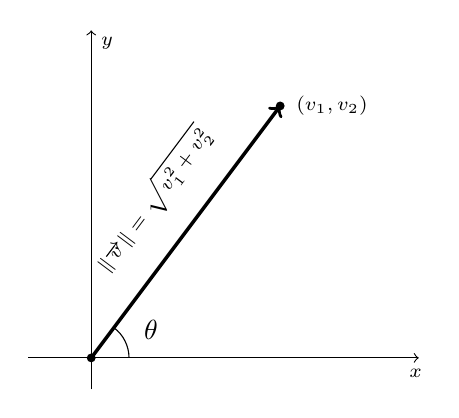
\begin{tikzpicture}[scale=0.8]

% Axes
\draw[->] (-1,0) -- (5.2,0);
\draw[->] (0,-0.5) -- (0,5.2);

% Axis labels
\node at (5.15,-0.25) {\scriptsize $x$};
\node at (0.25,5.0) {\scriptsize $y$};

% Angle theta
\draw (0.6,0) arc[start angle=0,end angle=53.13,radius=0.6];
\node at (0.95,0.45) {$\theta$};

% Length label
\node[rotate=53.13] at (1,2.5)
    {\scriptsize $\|\overrightarrow{v}\|=\sqrt{v_1^2+v_2^2}$};

% Endpoints
\fill (0,0) circle (2pt);
\fill (3,4) circle (2pt);

% Vector
\draw[->,line width=1.25pt] (0,0) -- (3,4);

% Endpoint label
\node[right] at (3.1,4)
    {\scriptsize $\left(v_1,v_2\right)$};

\end{tikzpicture}

\[
\overrightarrow{v}=\langle v_1,v_2\rangle
\text{ in standard position.}
\]
\end{center}

\phantomsection
\label{polarformvectorsection} 

Plotting a vector in standard position enables us to more easily quantify the concepts of magnitude and direction of the vector. 

 

Recall the magnitude of vector $\overrightarrow{v}$ is the length of the directed line segment representing $\overrightarrow{v}$.   When plotted in standard position, the length of this line segment  is none other than the distance from the origin $(0,0)$ to the point $\left(v_1,v_2\right)$.  Hence, the magnitude of $\overrightarrow{v}$, which we denote $\| \overrightarrow{v} \|$, is given by $\| \overrightarrow{v} \| = \sqrt{v_1^2 + v_2^2}$.

 

Turning to the notion of direction, we note that the point  $\left(v_1,v_2\right)$ is on the terminal side of the angle $\theta$ depicted in the diagram above.   From Theorem \ref{cosinesinecircle}, we have $v_1 = \| \overrightarrow{v} \| \cos(\theta)$ and $v_2  =  \| \overrightarrow{v} \| \sin(\theta)$. From the definition of scalar multiplication and vector equality, we get

\[ \begin{array}{rcl} \overrightarrow{v} & = & \left< v_1 , v_2  \right> \\   
															& = & \left< \| \overrightarrow{v} \| \cos(\theta), \| \overrightarrow{v} \| \sin(\theta) \right> \\   
													    & = &  \| \overrightarrow{v} \| \left< \cos(\theta),\sin(\theta) \right> \\ \end{array} \]
This motivates the following definition.

 

%% \colorbox{ResultColor}{\bbm
\begin{definition} \label{polarformvector}  Suppose $\overrightarrow{v}$ is a vector with component form $\overrightarrow{v} =\left< v_1 , v_2  \right>$.  Let $\theta$ be an angle in standard position whose terminal side contains the point $\left(v_1,v_2\right)$.

\begin{itemize}

\item  The \index{vector ! magnitude ! definition of} \textbf{magnitude} of $\overrightarrow{v}$, denoted $\| \overrightarrow{v} \|$, is given by $\| \overrightarrow{v} \| =   \sqrt{v_1^2 + v_2^2}$

\item If $\overrightarrow{v} \neq \overrightarrow{0}$, \index{vector ! direction ! definition of} the \textbf{(vector) direction} of $\overrightarrow{v}$, denoted $\hat{v}$ is given by  $\hat{v} = \left< \cos(\theta), \sin(\theta) \right>$

\end{itemize}

Taken together, we get $\overrightarrow{v} =  \left< \| \overrightarrow{v} \| \cos(\theta), \| \overrightarrow{v} \| \sin(\theta) \right>$.

\end{definition}
%% \ebm}

 

A few remarks are in order.   First, we note that if  $\overrightarrow{v} \neq 0$ then  there are infinitely many  angles $\theta$ which satisfy Definition \ref{polarformvector}.   However, the fact that all of them must contain the same point $\left(v_1,v_2\right)$  on their terminal sides means they are all coterminal.  

 

Hence, if $\theta$ and $\theta'$ both satisfy the conditions of Definition \ref{polarformvector}, then $\cos(\theta) = \cos(\theta')$ and $\sin(\theta) = \sin(\theta')$, and as such, $ \left< \cos(\theta), \sin(\theta) \right> =  \left< \cos(\theta'), \sin(\theta') \right>$ making $\hat{v}$ is well-defined.

 

For $\overrightarrow{0} = \left< 0, 0 \right>$, note that  $\| \overrightarrow{0} \| = \sqrt{0^2 + 0^2} = 0$.  Hence, $\| \overrightarrow{0} \|  \left< \cos(\theta), \sin(\theta) \right> = 0 \left< \cos(\theta), \sin(\theta) \right>  = <0,0>$ for \textit{every} angle $\theta$.  In other words, every angle $\theta$ satisfies the equation $\overrightarrow{v} =  \left< \| \overrightarrow{v} \| \cos(\theta), \| \overrightarrow{v} \| \sin(\theta) \right>$  in  Definition \ref{polarformvector}, so for this reason,  $\hat{0}$ is undefined. 

 

The following theorem summarizes the important facts about the magnitude and direction of a vector.

 


%% \colorbox{ResultColor}{\bbm
\begin{theorem}  \label{magdirprops}  \textbf{Properties of Magnitude and Direction}: Suppose $\overrightarrow{v}$ is a vector. \index{vector ! magnitude ! properties of} \index{vector ! direction ! properties of}

\begin{itemize}

\item $\| \overrightarrow{v} \| \geq 0$ and $\| \overrightarrow{v} \| = 0$ if and only if $\overrightarrow{v} = \overrightarrow{0}$

\item  For all scalars $k$,  $\| k \, \overrightarrow{v} \| = |k| \| \overrightarrow{v} \|$.

\item  If $\overrightarrow{v} \neq \overrightarrow{0}$ then $\overrightarrow{v} = \| \overrightarrow{v} \| \hat{v}$, so that $\hat{v} = \left(\frac{1}{\|\overrightarrow{v}\|}\right) \overrightarrow{v}$.

\end{itemize}

\end{theorem}

 

%% \ebm}

 

The proof of the first property in Theorem \ref{magdirprops} is a direct consequence of the definition of $\| \overrightarrow{v} \|$.  Given $\overrightarrow{v}  = \left< v_1 ,v_2\right>$, then $\| \overrightarrow{v} \| = \sqrt{v_1^2 + v_2^2}$ which is by definition greater than or equal to $0$.  Moreover, $\sqrt{v_1^2 + v_2^2} = 0$ if and only of $v_1^2 + v_2^2 = 0$ if and only if $v_1 = v_2 = 0$.  Hence, $\| \overrightarrow{v} \| = 0$ if and only if $\overrightarrow{v} = \left<0,0\right> =  \overrightarrow{0}$, as required.

 

The second property is a result of the definition of magnitude and scalar multiplication along with a property of radicals. If $\overrightarrow{v} = \left< v_1 ,v_2\right>$ and $k$ is a scalar then 

\[ \begin{array}{rcll}

\| k \, \overrightarrow{v} \| & = & \| k \left< v_1, v_2\right> \| & \\   
									 & = & \| \left<kv_1,kv_2\right>\| & \text{Definition of scalar multiplication} \\   
									 & = & \sqrt{\left(kv_1\right)^2 + \left(kv_2\right)^2} & \text{Definition of magnitude} \\   
									 & = & \sqrt{k^2v_1^2 + k^2v_2^2} & \\  
									 & = & \sqrt{k^2(v_1^2+v_2^2)} & \\   
									 & = & \sqrt{k^2} \sqrt{v_1^2+v_2^2} & \text{Product Rule for Radicals} \\   
									 & = & |k| \sqrt{v_1^2+v_2^2} & \text{Since $\sqrt{k^2} = |k|$} \\
									 & = & |k| \| \overrightarrow{v} \| & \\
\end{array} \]

 

The equation $\overrightarrow{v} = \| \overrightarrow{v} \| \hat{v}$ in Theorem \ref{magdirprops} is a consequence of the definitions of $\| \overrightarrow{v} \|$ and $\hat{v}$ and was worked out in the discussion just prior to Definition \ref{polarformvector} on page \pageref{polarformvectorsection}.  In words, the equation $\overrightarrow{v} = \| \overrightarrow{v} \| \hat{v}$  says that any given vector is the product of its magnitude and its direction -- an important concept to keep in mind when studying and using vectors. 

 

The formula for   $\hat{v}$ stated  in Theorem \ref{magdirprops}  is a consequence of solving $\overrightarrow{v} = \| \overrightarrow{v} \| \hat{v}$  for $\hat{v}$ by multiplying\footnote{Of course, to go from $\overrightarrow{v} = \| \overrightarrow{v} \| \hat{v}$ to $\hat{v} = \left( \frac{1}{\|\overrightarrow{v}\|}\right) \overrightarrow{v}$, we are essentially `dividing both sides' of the equation by the scalar $\| \overrightarrow{v} \|$.  The authors encourage the reader, however, to work out the details carefully to gain an appreciation of the properties in play.} both sides of the equation by $\frac{1}{\| \overrightarrow{v} \|}$ and using the properties of Theorem \ref{vectorscalarmultprops}.  We leave these details to the reader. We are overdue for an example.

\newpage

\begin{example} \label{polarformvecex} $~$

\begin{enumerate}

\item \label{resolvecomponents} Find the component form of the vector $\overrightarrow{v}$ with $\|\overrightarrow{v}\| = 5$ so that when $\overrightarrow{v}$ is plotted in standard position, it lies in Quadrant II and makes a $60^{\circ}$ angle\footnote{Due to the utility of vectors in `real-world' applications, we will usually use degree measure for the angle when giving the vector's direction.  That being said, since Carl doesn't want you to forget about radians, he's made sure there are examples and exercises which use them as well.} with the negative $x$-axis.

\item  For $\overrightarrow{v} = \left<3, -3\sqrt{3}\right>$, find $\|\overrightarrow{v}\|$ and $\theta$, $0 \leq \theta < 2\pi$ so that $\overrightarrow{v} = \| \overrightarrow{v} \| \left<\cos(\theta), \sin(\theta)\right>$.

\item For the vectors $\overrightarrow{v} = \left<3,4\right>$ and $\overrightarrow{w} = \left<1, -2\right>$, find the following.

\begin{multicols}{4}

\begin{enumerate}

\item  $\hat{v}$

\item  $\| \overrightarrow{v} \| -2 \|\overrightarrow{w}\|$

\item  $\| \overrightarrow{v} -2\overrightarrow{w}\|$

\item  $\| \hat{w} \|$ \label{preludetounitvector}

\end{enumerate}

\end{multicols}

\end{enumerate}

\begin{explanation}

\begin{enumerate}

\item  We are told that $\| \overrightarrow{v} \| = 5$ and are given information about its direction, so we can use the formula $\overrightarrow{v} = \| \overrightarrow{v} \| \hat{v}$ to get the component form of $\overrightarrow{v}$. 

 

 To determine $\hat{v}$, we appeal to Definition \ref{polarformvector}.  Since $\overrightarrow{v}$ lies in Quadrant II and makes a  $60^{\circ}$ angle with the negative $x$-axis, one angle $\theta$ satisfying the criteria of  Definition \ref{polarformvector} is $\theta = 120^{\circ}$.  
 

\begin{center}
\begin{tikzpicture}[scale=0.8]

% Axes
\draw[->] (-4.2,0) -- (4.2,0);
\draw[->] (0,-1.2) -- (0,6.2);

% Tick marks and labels on x-axis
\foreach \x in {-3,-2,-1,1,2,3}{
    \draw (\x,0.08) -- (\x,-0.08);
    \node[below] at (\x,-0.08) {\scriptsize $\x$};
}

% Tick marks and labels on y-axis
\foreach \y in {1,2,3,4,5}{
    \draw (0.08,\y) -- (-0.08,\y);
    \node[left] at (-0.08,\y) {\scriptsize $\y$};
}

% Axis labels
\node at (4,-0.35) {\scriptsize $x$};
\node at (0.3,6) {\scriptsize $y$};

% Angle arcs
\draw[->] (1.2,0) arc[start angle=0,end angle=120,radius=1.2];
\draw[<->] (-0.6,1.04) arc[start angle=120,end angle=180,radius=1.2];

% Angle labels
\node at (2.5,1) {\scriptsize $\theta=120^\circ$};
\node at (-2,1) {\scriptsize $60^\circ$};

% Vector
\draw[->,line width=1.25pt] (0,0) -- (-2.5,4.33);

% Vector label
\node at (-1.25,3) {\scriptsize $\overrightarrow{v}$};

\end{tikzpicture}
\end{center}

Hence,  $\hat{v} = \left< \cos\left(120^{\circ}\right), \sin\left(120^{\circ}\right) \right> = \left< - \frac{1}{2} , \frac{\sqrt{3}}{2} \right>$, so  $\overrightarrow{v} = \| \overrightarrow{v} \| \hat{v} = 5  \left< - \frac{1}{2} , \frac{\sqrt{3}}{2} \right> =  \left< - \frac{5}{2} , \frac{5\sqrt{3}}{2} \right>$.


\item  For $\overrightarrow{v} =  \left<3, -3\sqrt{3}\right>$, we get $\| \overrightarrow{v} \| = \sqrt{(3)^2+(-3\sqrt{3})^2} = 6$.  In light of Definition \ref{polarformvector}, we can find the $\theta$ we're after by finding a Quadrant IV angle whose terminal side contains the point  $(3, -3\sqrt{3})$.  

 

Going through the usual calculations, we find $\cos(\theta) = \frac{1}{2}$ and $\sin(\theta) = -\frac{\sqrt{3}}{2}$.  Hence,  $\theta = \frac{5\pi}{3}$.  

 

We may check our answer by verifying $6\left<\cos\left(\frac{5\pi}{3}\right), \sin\left(\frac{5\pi}{3}\right) \right>  = \left<3, -3\sqrt{3}\right> = \overrightarrow{v}$.

\item  \begin{enumerate} \item  Since we are given the component form of $\overrightarrow{v}$, we'll use the formula $\hat{v} = \left(\frac{1}{\|\overrightarrow{v}\|}\right) \overrightarrow{v}$.  For $\overrightarrow{v} = \left<3,4\right>$, we have $\| \overrightarrow{v} \| = \sqrt{3^2+4^2} = \sqrt{25} = 5$.  Hence, $\hat{v} = \frac{1}{5} \left< 3, 4 \right> = \left<\frac{3}{5}, \frac{4}{5}\right>$.


\item  We know from our work above that $\| \overrightarrow{v} \| = 5$, so to find  $\| \overrightarrow{v} \| -2 \|\overrightarrow{w}\|$, we need only find $\| \overrightarrow{w} \|$.  Since $\overrightarrow{w} = \left<1, -2\right>$, we get $\| \overrightarrow{w} \| = \sqrt{1^2+(-2)^2} = \sqrt{5}$.  Hence, $\| \overrightarrow{v} \| -2 \|\overrightarrow{w}\| = 5 - 2\sqrt{5}$.

\item  In the expression $\| \overrightarrow{v} -2\overrightarrow{w}\|$, notice that the arithmetic on the vectors comes first, then the magnitude.  Hence, our first step is to find the component form of the vector $\overrightarrow{v} - 2\overrightarrow{w}$.  We get $\overrightarrow{v} - 2 \overrightarrow{w} = \left<3,4\right> - 2\left<1,-2\right> = \left<1, 8\right>$.  Hence,  $\| \overrightarrow{v} -2\overrightarrow{w}\| =  \| \left<1, 8\right>\| = \sqrt{1^2+8^2} = \sqrt{65}$.

\item  One approach to find $\| \hat{w} \|$, is to first find $\hat{w}$ and then take the magnitude.

 

Using the formula  $\hat{w} = \left(\frac{1}{\| \overrightarrow{w} \|}\right) \overrightarrow{w}$ along with $\| \overrightarrow{w} \| = \sqrt{5}$, which we found the in the previous problem, we get  $\hat{w} = \frac{1}{\sqrt{5}} \left<1, -2\right> = \left< \frac{1}{\sqrt{5}}, -\frac{2}{\sqrt{5}}\right>  = \left< \frac{\sqrt{5}}{5}, -\frac{2\sqrt{5}}{5}\right>$.   

 

Hence, $\| \hat{w} \| = \sqrt{\left( \frac{\sqrt{5}}{5}\right)^2 + \left(-\frac{2\sqrt{5}}{5}\right)^2} = \sqrt{\frac{5}{25} + \frac{20}{25}} = \sqrt{1} = 1$. 

Alternatively, we can use Theorem \ref{magdirprops}.  Since $\hat{w} = \left(\frac{1}{\| \overrightarrow{w} \|} \right) \overrightarrow{w}$, where $\frac{1}{\| \overrightarrow{w} \|}>0$ is a scalar,   \[ \| \hat{w} \| = \left\|  \left(\frac{1}{\| \overrightarrow{w} \|} \right) \overrightarrow{w} \right\| = \frac{1}{\| \overrightarrow{w} \|} \| \overrightarrow{w} \| = \frac{\| \overrightarrow{w} \|}{\| \overrightarrow{w} \|} = 1.\] 

For a third way to show $\| \hat{w} \| = 1$, we can appeal to Definition \ref{polarformvector}.  Since $\hat{w} = \left< \cos(\theta), \sin(\theta) \right>$ for some angle $\theta$, $\| \hat{w} \| = \sqrt{\cos^{2}(\theta) + \sin^{2}(\theta)} = \sqrt{1} = 1$, where we have used the Pythagorean Identity, $\cos^{2}(\theta) + \sin^{2}(\theta) = 1$.  No matter how we approach the problem, $\| \hat{w} \| = 1$. \qed


\end{enumerate}

\end{enumerate}
\end{explanation}
\end{example}

Note that the second and third solutions to number \ref{preludetounitvector} in Example \ref{polarformvecex} above work for \textit{any} nonzero vector, $\overrightarrow{w}$.  We will have more to say about this shortly.

The process exemplified by number \ref{resolvecomponents} in Example \ref{polarformvecex} above by which we take information about the magnitude and direction of a vector and find the component form of a vector is called \textbf{resolving} a vector into its components.  As an application of this process, we revisit Example \ref{vectorbearingex} below.


\begin{example} \label{vectorbearingexresolve}  A plane leaves an airport with an airspeed of 175 miles per hour with bearing N$40^{\circ}$E.  A 35 mile per hour wind is blowing at a bearing of S$60^{\circ}$E.  Find the true speed of the plane, rounded to the nearest mile per hour,  and the true bearing of the plane, rounded to the nearest degree.

\begin{explanation}
We proceed as we did in Example \ref{vectorbearingex} and let $\overrightarrow{v}$ denote the plane's velocity and $\overrightarrow{w}$ denote the wind's velocity, and set about determining $\overrightarrow{v} + \overrightarrow{w}$.  

 

If we regard the airport as being at the origin, the positive $y$-axis acting as due north and the positive $x$-axis acting as due east, we see that the vectors $\overrightarrow{v}$ and $\overrightarrow{w}$ are in standard position and their directions correspond to the angles $50^{\circ}$ and $-30^{\circ}$, respectively.  

 

Hence, the component form of $\overrightarrow{v} = 175\left<\cos(50^{\circ}), \sin(50^{\circ})\right> = \left<175\cos(50^{\circ}), 175\sin(50^{\circ})\right>$ and the component form of $\overrightarrow{w} = \left<35\cos(-30^{\circ}), 35\sin(-30^{\circ}) \right>$.  

 

Since we have no convenient way to express the exact values of cosine and sine of $50^{\circ}$, we leave both vectors in terms of cosines and sines.\footnote{Keeping things `calculator' friendly, for once!}  Adding corresponding components, we find the resultant vector $\overrightarrow{v} + \overrightarrow{w} = \left< 175\cos(50^{\circ}) + 35\cos(-30^{\circ}), 175\sin(50^{\circ}) + 35\sin(-30^{\circ})\right>$.  To find the `true' speed of the plane, we compute the magnitude of this resultant vector

\[ \| \overrightarrow{v} + \overrightarrow{w}\| = \sqrt{ (175\cos(50^{\circ}) + 35\cos(-30^{\circ}))^2 + (175\sin(50^{\circ}) + 35\sin(-30^{\circ}))^2} \approx 184\]

Hence, the `true' speed of the plane is approximately 184 miles per hour. 

 

 To find the true bearing, we need to find the angle $\theta$  whose terminal side when graphed in standard position contains $(x,y) = (175\cos(50^{\circ}) + 35\cos(-30^{\circ}), 175\sin(50^{\circ}) + 35\sin(-30^{\circ}))$.  
 
  
 
 Since both of these coordinates are positive,\footnote{Yes, a calculator approximation is the quickest way to see this, but you can also use good old-fashioned inequalities and the fact that $45^{\circ} \leq 50^{\circ} \leq 60^{\circ}$.} we know $\theta$ is a Quadrant I angle, as depicted below.  Furthermore, \[\tan(\theta) = \frac{y}{x} = \frac{175\sin(50^{\circ}) + 35\sin(-30^{\circ})}{175\cos(50^{\circ}) + 35\cos(-30^{\circ})},\]

so using the arctangent function,\footnote{We could just have easily used arcsine or arccosine here \ldots} we get $\theta \approx 39^{\circ}$.  Since, for the purposes of bearing, we need the angle between $\overrightarrow{v} + \overrightarrow{w}$ and the positive $y$-axis, we take the complement of $\theta$ and find the `true' bearing of the plane to be approximately N$51^{\circ}$E.

\[
\begin{array}{cc}

\begin{tikzpicture}[scale=0.6]

% Axes
\draw[->] (-1,0) -- (8.3,0);
\draw[->] (0,-2.2) -- (0,9.3);

% Axis labels
\node[anchor=west] at (8,-0.5) {\scriptsize $x$ (E)};
\node[anchor=west] at (0.5,9) {\scriptsize $y$ (N)};

% Angle arcs
\draw[->] (0,3) ++(85:0) arc[start angle=85,end angle=45,radius=3];
\node at (1.2,3.3) {\scriptsize $40^\circ$};

\draw[->] (3,0) arc[start angle=5,end angle=45,radius=3];
\node at (3.2,1.5) {\scriptsize $50^\circ$};

\draw[->] (0,1.5) ++(275:0) arc[start angle=275,end angle=325,radius=1.5];
\node at (1,-1.73) {\scriptsize $60^\circ$};

\draw[->] (1.5,0) arc[start angle=-5,end angle=-25,radius=1.5];
\node at (2.3,-0.52) {\scriptsize $-30^\circ$};

% Vectors
\draw[->,line width=1.25pt] (0,0)--(6.43,7.66);
\node at (6.75,8.04) {\scriptsize $\vec v$};

\draw[->,line width=1.25pt] (0,0)--(1.73,-1);
\node at (2.16,-1.25) {\scriptsize $\vec w$};

\end{tikzpicture}

&\quad
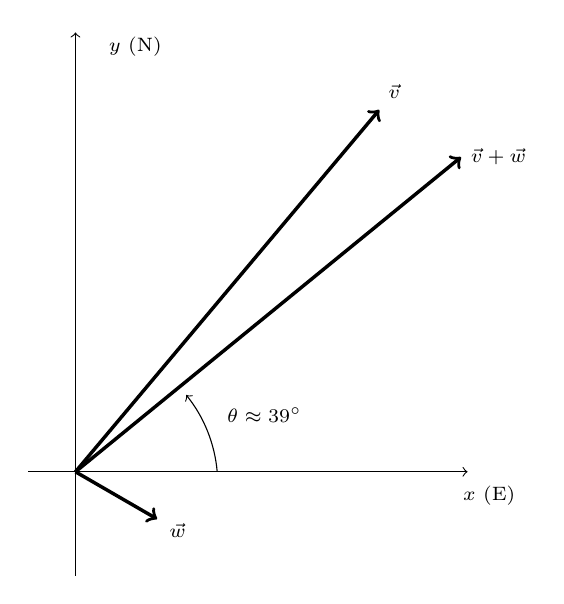
\begin{tikzpicture}[scale=0.6]

% Axes
\draw[->] (-1,0) -- (8.3,0);
\draw[->] (0,-2.2) -- (0,9.3);

% Axis labels
\node[anchor=west] at (8,-0.5) {\scriptsize $x$ (E)};
\node[anchor=west] at (0.5,9) {\scriptsize $y$ (N)};

% Resultant angle
\draw[->] (3,0) arc[start angle=5,end angle=39,radius=3];
\node at (4,1.2) {\scriptsize $\theta\approx39^\circ$};

% Vectors
\draw[->,line width=1.25pt] (0,0)--(6.43,7.66);
\node at (6.75,8.04) {\scriptsize $\vec v$};

\draw[->,line width=1.25pt] (0,0)--(1.73,-1);
\node at (2.16,-1.25) {\scriptsize $\vec w$};

\draw[->,line width=1.25pt] (0,0)--(8.16,6.66);
\node[right] at (8.16,6.66) {\scriptsize $\vec v+\vec w$};

\end{tikzpicture}
\end{array}
\]
%\arrow \dashed \polyline{(0,0), (8.16,6.66)}
%\dotted \polyline{(1.73, -1), (8.16, 6.66)}
%\dotted \polyline{(6.43, 7.66), (8.16, 6.66)}
%\tlabel[cc](9,6.75){\scriptsize $\overrightarrow{v} + \overrightarrow{w}$}
\end{explanation} 
\end{example}

In part \ref{preludetounitvector} of Example \ref{polarformvecex}, we saw that the length of the direction vector, $\hat{w}$,  $\| \hat{w} \| = 1$.  Vectors of length $1$  play such an important role that they are given a special name.

 

%% \colorbox{ResultColor}{\bbm
\begin{definition} \label{unitvectordefn} \index{vector ! unit vector} \index{unit vector} \textbf{Unit Vectors:}   Let $\overrightarrow{v}$ be a vector. If $\| \overrightarrow{v} \| = 1$, we say that $\overrightarrow{v}$ is a \textbf{unit vector}.

\end{definition}
%% \ebm}
 

Note that if $\overrightarrow{v}$ is a unit vector, then necessarily,  $\overrightarrow{v} = \| \overrightarrow{v} \| \hat{v} = 1 \cdot \hat{v} = \hat{v}$.  Conversely,  in the solution of part \ref{preludetounitvector} of Example \ref{polarformvecex}, two different arguments show for any nonzero vector $\overrightarrow{v}$, $\| \hat{v} \| = 1$, so $\hat{v}$ is a unit vector.  

 

In other words, unit vectors are direction vectors and vice-versa. Indeed, the vector $\hat{v}$ which we have defined as `the \textit{direction} of $\overrightarrow{v}$' is often described as `the \textit{unit vector in the direction} of $\overrightarrow{v}$.'

 

  In practice, if $\overrightarrow{v}$ is a unit vector we write it as $\hat{v}$ as opposed to $\overrightarrow{v}$ because we have reserved the `$\hat{~}$' notation for unit vectors.  The process of multiplying a nonzero vector by the factor $\frac{1}{\| \overrightarrow{v} \|}$ to produce a unit vector is called \index{vector ! normalization} `\textbf{normalizing} the vector.'  
  
   
  
   The terminal points of unit vectors, when plotted in standard position, lie on the Unit Circle. (You should take the time to show this.)  As a result, we visualize normalizing a nonzero vector $\overrightarrow{v}$ as shrinking\footnote{\ldots if $\| \overrightarrow{v} \| > 1$ \ldots} its terminal point, when plotted in standard position, back to the Unit Circle.

\begin{center}

\begin{tikzpicture}[scale=0.8]

% Unit circle
\draw[gray!70] (0,0) circle (2);

% Axes
\draw[->] (-4.2,0) -- (4.2,0);
\draw[->] (0,-4.2) -- (0,4.2);

% Tick marks
\foreach \x/\lbl in {-2/-1,2/1}{
    \draw (\x,0.08) -- (\x,-0.08);
    \node[below] at (\x,-0.08) {\scriptsize $\lbl$};
}

\foreach \y/\lbl in {-2/-1,2/1}{
    \draw (0.08,\y) -- (-0.08,\y);
    \node[left] at (-0.08,\y) {\scriptsize $\lbl$};
}

% Axis labels
\node[anchor=west] at (4,-0.45) {\scriptsize $x$};
\node[anchor=west] at (0.3,4) {\scriptsize $y$};

% Vector v
\draw[->,line width=1.25pt] (0,0) -- (2,3.46);
\node[right] at (2,3.46) {$\overrightarrow{v}$};

% Unit vector v-hat
\draw[->,line width=1.0pt] (0,0) -- (1,1.73);
\node at (1.45,1.73) {$\hat{v}$};

\end{tikzpicture}

\vspace{1ex}

Visualizing vector normalization
\[
\hat{v}
=
\left(\frac{1}{\|\overrightarrow{v}\|}\right)\overrightarrow{v}.
\]

\end{center}

Of all of the unit vectors, two deserve special mention.

 

%% \colorbox{ResultColor}{\bbm

\begin{definition} \label{ihatjhatdefn}  \textbf{The Principal Unit Vectors:} $~$ \index{vector ! principal unit vectors, $\hat{\text{i}}$, $\hat{\text{j}}$} \index{principal unit vectors, $\hat{\text{i}}$, $\hat{\text{j}}$} 

\begin{itemize}

\item The vector $\hat{\text{i}}$ is defined by $\hat{\text{i}} = \left<1,0\right>$

\item The vector $\hat{\text{j}}$ is defined by $\hat{\text{j}} = \left<0,1\right>$

\end{itemize}

 

\end{definition}

%% \ebm}

 

Geometrically, in the $xy$-plane, the vector $\hat{\text{i}}$ as represents the positive $x$-direction, whereas the vector $\hat{\text{j}}$ represents the positive $y$-direction.  We have the following `decomposition' theorem.\footnote{We will see a generalization of Theorem \ref{ijdecomp} in Section \ref{TheDotProduct}.  Stay tuned!}  

 

%% \colorbox{ResultColor}{\bbm

\begin{theorem} \label{ijdecomp}  \textbf{Principal Vector Decomposition Theorem:} 

 Let $\overrightarrow{v}$ be a vector with component form  $\overrightarrow{v} = \left< v_1 ,v_2\right>$. Then $\overrightarrow{v} = v_1 \hat{\text{i}} + v_2 \hat{\text{j}}$. \index{vector ! Decomposition Theorem ! Principal}


\end{theorem}

%% \ebm}

 

The proof of Theorem \ref{ijdecomp} is straightforward. Since $\hat{\text{i}} = \left<1,0\right>$ and $\hat{\text{j}} = \left< 0,1\right>$, we have from the definition of scalar multiplication and vector addition that  

\[v_1 \hat{\text{i}} + v_2 \hat{\text{j}} = v_1\left<1,0\right> + v_2\left<0,1\right> = \left<v_1,0\right> + \left<0,v_2\right> = \left<v_1,v_2\right> = \overrightarrow{v}\]

Geometrically, the situation looks like this:


\begin{center}
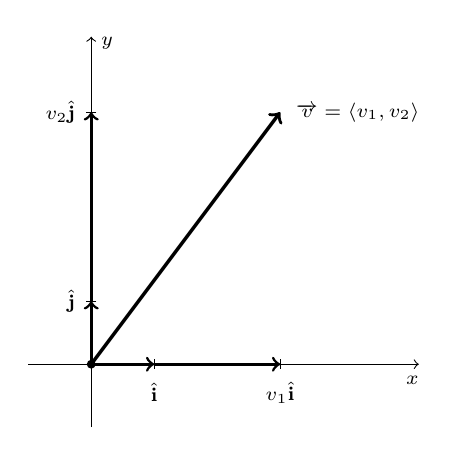
\begin{tikzpicture}[scale=0.8]

% Axes
\draw[->] (-1,0) -- (5.2,0);
\draw[->] (0,-1) -- (0,5.2);

% Tick marks
\foreach \x in {1,3}
    \draw (\x,0.08) -- (\x,-0.08);

\foreach \y in {1,4}
    \draw (0.08,\y) -- (-0.08,\y);

% Axis labels
\node at (5.1,-0.25) {\scriptsize $x$};
\node at (0.25,5.1) {\scriptsize $y$};

% Origin
\fill (0,0) circle (2pt);

% Vector v
\draw[->,line width=1.25pt] (0,0) -- (3,4);
\node[right] at (3.1,4)
    {\scriptsize $\overrightarrow{v}=\langle v_1,v_2\rangle$};

% x-component
\draw[->,line width=1pt] (0,0) -- (1,0);
\draw[->,line width=1pt] (1,0) -- (3,0);

% y-component
\draw[->,line width=1pt] (0,0) -- (0,1);
\draw[->,line width=1pt] (0,1) -- (0,4);

% Labels
\node at (1,-0.45) {\scriptsize $\hat{\mathbf{i}}$};
\node at (3,-0.45) {\scriptsize $v_1\hat{\mathbf{i}}$};

\node[left] at (-0.1,1) {\scriptsize $\hat{\mathbf{j}}$};
\node[left] at (-0.1,4) {\scriptsize $v_2\hat{\mathbf{j}}$};

\end{tikzpicture}

\vspace{0.5em}

$\displaystyle
\overrightarrow{v}
=\langle v_1,v_2\rangle
=
v_1\hat{\mathbf{i}}
+
v_2\hat{\mathbf{j}}.
$

\end{center}

We conclude this section with a classic example which demonstrates how vectors are used in physics to study forces.  A `force' is defined as a `push' or a `pull.'   The intensity of the push or pull is the magnitude of the force, and is  measured in Netwons (N) in the SI system or pounds (lbs.)$\!$ in the English system.\footnote{See also Section \ref{harmomicmotion}.} 

 

 The following example uses all of the concepts in this section, and should be studied in great detail.

\begin{example} \label{forceex}  A $50$ pound speaker is  suspended from the ceiling by two support braces.   If one of them makes a $60^{\circ}$ angle with the ceiling and the other makes a $30^{\circ}$ angle with the ceiling, what are the tensions on each of the supports?

\begin{explanation}
We represent the problem schematically below along with  the corresponding vector diagram. 

\begin{center}
\begin{tikzpicture}[scale=0.7]

%========================
% Left picture
%========================
\begin{scope}

% Ceiling
\fill[pattern=north east lines,pattern color=gray!70]
    (-8,4) rectangle (3,5);
\draw (-8,4) rectangle (3,5);

% Block
\draw (-2,-4) rectangle (2,0);

% Cables
\draw (0,0)--(2.31,4);
\draw (0,0)--(-6.93,4);

% Angles
\draw[<->] (2.31,4) ++(185:1.5)
    arc[start angle=185,end angle=235,radius=1.5];

\draw[<->] (-6.93,4) ++(-5:2)
    arc[start angle=-5,end angle=-25,radius=2];

% Labels
\node at (-4,3.25) {$30^\circ$};
\node at (0,3.25) {$60^\circ$};
\node at (0,-2) {50 lbs.};

% Points
\fill (0,0) circle (2pt);
\fill (-6.93,4) circle (2pt);
\fill (2.31,4) circle (2pt);

\end{scope}


%========================
% Right picture
%========================
\begin{scope}[xshift=12cm]

% Dotted original vectors
\draw[dotted] (0,0)--(-6.93,4);
\draw[dotted] (0,0)--(2.31,4);
\draw[dotted] (-8,4)--(3,4);

% Horizontal reference
\draw[dashed] (-8,0)--(3,0);

% Tension vectors
\draw[->,line width=1.25pt]
    (0,0)--({4*cos(60)},{4*sin(60)});

\draw[->,line width=1.25pt]
    (0,0)--({4*cos(150)},{4*sin(150)});

% Weight vector
\draw[->,line width=1.25pt]
    (0,0)--(0,-4);

% Angle labels
\node at (-4,3.25) {$30^\circ$};
\node at (0,3.25) {$60^\circ$};

\node at (-2.1,0.5) {$30^\circ$};
\node at (2.3,1) {$60^\circ$};

% Vector labels
\node at (0.5,-2) {$\overrightarrow{w}$};
\node at (2.5,3.4) {$\overrightarrow{T_1}$};
\node at (-3,2.25) {$\overrightarrow{T_2}$};

% Angle arcs at origin
\draw[<->] (2,0) arc[start angle=0,end angle=60,radius=2];
\draw[<->] (-1.25,.675) arc[start angle=150,end angle=180,radius=1.5];

% Joint
\fill (0,0) circle (2pt);

\end{scope}

\end{tikzpicture}
\end{center}

 We have three forces acting on the speaker:  the weight of the speaker, which we'll call  $\overrightarrow{w}$, pulling the speaker directly downward, and the forces on the support rods, which we'll call $\overrightarrow{T_1}$ and $\overrightarrow{T_2}$ (for `tensions') acting upward at angles $60^{\circ}$ and $30^{\circ}$, respectively.  
 
  
 
 We are looking for the tensions on the support, which are the magnitudes  $\| \overrightarrow{T_1} \|$  and  $\| \overrightarrow{T_2} \|$.   In order for the speaker to remain stationary,\footnote{This is the criteria for `static equilbrium'.} we require  $\overrightarrow{w} + \overrightarrow{T_1} + \overrightarrow{T_2} = \overrightarrow{0}$.  
 
  
 
 Viewing the common initial point of these vectors as the origin and the dashed line as the $x$-axis, we use Theorem \ref{magdirprops} to get component representations for the three vectors involved. We can model the weight of the speaker as a vector pointing directly downwards with a magnitude of 50 pounds.  That is,  $\| \overrightarrow{w} \| = 50$ and $\hat{w} = -\hat{\text{j}} = \left<0,-1\right>$.  Hence, $\overrightarrow{w} = 50\left<0,-1\right> = \left<0,-50\right>$.  For the force in the first support, we get
 
\[ \begin{array}{rcl}

 \overrightarrow{T_1} &  = &  \| \overrightarrow{T_1} \|\left<\cos\left(60^{\circ}\right), \sin\left(60^{\circ}\right)\right> \\   
                            & =  & \left< \frac{\| \overrightarrow{T_1} \|}{2} , \frac{\| \overrightarrow{T_1} \|\sqrt{3}}{2}\right> \\ \end{array} \]
                            
For the second support, we note that the angle $30^{\circ}$ is measured from the negative $x$-axis, so the angle needed to write $\overrightarrow{T_2}$ in component form is $150^{\circ}$.  Hence

\[ \begin{array}{rcl}

\overrightarrow{T_2} & = & \| \overrightarrow{T_2} \|\left<\cos\left(150^{\circ}\right), \sin\left(150^{\circ}\right)\right>\\   
                           & =  & \left<-\frac{\| \overrightarrow{T_2} \|\sqrt{3}}{2}, \frac{\| \overrightarrow{T_2} \|}{2} \right> \\ \end{array} \]
                           
The requirement $\overrightarrow{w} + \overrightarrow{T_1} + \overrightarrow{T_2} = \overrightarrow{0}$ gives us the vector equation:
 
 \[ \begin{array}{rcl}
 
\overrightarrow{w} + \overrightarrow{T_1} + \overrightarrow{T_2} &  = &  \overrightarrow{0}  \\   

\left<0,-50\right> + \left< \frac{\| \overrightarrow{T_1} \|}{2} , \frac{\| \overrightarrow{T_1} \|\sqrt{3}}{2}\right> +  \left<-\frac{\| \overrightarrow{T_2} \|\sqrt{3}}{2}, \frac{\| \overrightarrow{T_2} \|}{2} \right> & = & \left<0, 0\right> \\   

\left< \frac{\| \overrightarrow{T_1} \|}{2} -\frac{\| \overrightarrow{T_2} \|\sqrt{3}}{2}, \frac{\| \overrightarrow{T_1} \|\sqrt{3}}{2} +  \frac{\| \overrightarrow{T_2} \|}{2} -50  \right> & = & \left<0, 0\right>  \\ 
\end{array} \]

Equating the corresponding components of the vectors on each side,  we get a system of linear equations in the variables $\| \overrightarrow{T_1} \| $ and   $\| \overrightarrow{T_2} \|$.

\[\left\{ \begin{array}{lrcl} (E1) &  \frac{\| \overrightarrow{T_1} \|}{2} -\frac{\| \overrightarrow{T_2} \|\sqrt{3}}{2} & = & 0 \\     (E2) &  \frac{\| \overrightarrow{T_1} \|\sqrt{3}}{2} +  \frac{\| \overrightarrow{T_2} \|}{2} -50 & = & 0 \\ \end{array} \right.\]

From $(E1)$, we get $\| \overrightarrow{T_1} \| = \| \overrightarrow{T_2} \| \sqrt{3}$.  Substituting that into $(E2)$ gives $\frac{(\| \overrightarrow{T_2} \| \sqrt{3})\sqrt{3}}{2} +  \frac{\| \overrightarrow{T_2} \|}{2} - 50 = 0$.

 

Solving, we get  $2\| \overrightarrow{T_2} \| - 50 =0$, so  $\| \overrightarrow{T_2} \| = 25$ pounds.  Hence,   $\| \overrightarrow{T_1} \| = \| \overrightarrow{T_2} \| \sqrt{3} = 25 \sqrt{3}$ pounds.   \qed
\end{explanation}
\end{example}


Note that the sum of the tensions on the wires in Example \ref{forceex} exceed the $50$ pounds of the speaker.  Explaining why this happens is a good exercise and gets at the heart of the concept of vectors and resolution of forces.  Speaking of exercises \ldots


%% SKIPPED %% \input{ExercisesforVectors}

\closegraphsfile

\end{document}
